\documentclass[10pt]{article}
    \usepackage[left=1in, right=1in, top=1in, bottom=1in, nohead, nofoot]{geometry}
    \usepackage[utf8]{inputenc}
    \usepackage[english]{babel}
    \usepackage[document]{ragged2e}
    \usepackage{datetime} 
    \usepackage{amssymb}
    \usepackage{graphicx}
    \usepackage{cancel}
    \usepackage{hyperref}
    \pagenumbering{gobble}
\begin{document}
    \begin{center} 
        \large\textbf{ECI 149 HW 2}

        \normalsize Charles Reid Hammond \\ \today

    \end{center} 

    \setlength{\parskip}{\baselineskip}

    \begin{flushleft}

        \textbf{Problem 1:} 
        
        $\frac{3.4\times 10^9 barrel}{year} \times \frac{42 gal}{barrel} \times \frac{0.72 g-fuel}{ml}\times \frac{ml}{0.000264 gal}\times \frac{0.842 g-C}{g-fuel}=3.3\times 10^{14}g-C /year$

       $3.3\times 10^{11}kg-C /year \times 0.99 \times \frac{0.044kg-CO_2}{0.012kg-C}\times \frac{0.2 g-PM_{2.5}}{kg-CO_2}\times \frac{year}{365 days} \times \frac{1 metric\:ton}{1000000 g} = 652.2$ metric tons of $PM_{2.5}$ per day.


        \hrulefill


        \textbf{Problem 2:}

        a) $\frac{2.3\times 14.8 lb-ash}{ton-coal}\times \frac{3520\times 10^6 W}{33\%}\times \frac{BTU/hr}{0.293 W} \times \frac{ton-coal}{25\times 10^6 BTU} \times \frac{0.454 kg}{lb} = 22504.35 kg-ash/hr$

        b) 20704.0 kg/hr decrease.

        \hrulefill


        \textbf{Problem 3:}

        The equivalent standard at 14,505 ft would mean what concentration of $O_3$ will give you 70ppb by volume at that altitude.

        So:

        $\left(\frac{n}{V}\right)_{air}^{14,505ft}=\frac{1.0132\times 10^5 e^{\frac{-4.42km}{7.4km}}}{1.381\times 10^{-23}\times 281 K}\times (m/100cm)^3=1.437\times10^{19} molec/cm^3$

        And therefore,

        a)

        $70ppb=\frac{\left(\frac{n}{V}\right)_{O_3}}{\left(\frac{n}{V}\right)_{air}^{14,505ft}}\times 10^9\rightarrow \left(\frac{n}{V}\right)_{O_3} =1.0\times 10^{12} molec/cm^3 $

        b) mass density = $\left(\frac{n}{V}\right)_{O_3}\times 48 g/mol /\left(6.022\times 10^{23} molec/mol\right)\times 1000000 \mu g / g \times (100cm/m)^3 = 80.2 \mu g/m^3$

        \hrulefill


        \textbf{Problem 4:}

        High pressure systems involve air moving downward, which means the air warms and dries, so no precipitation occurs.

        Low pressure systems involve air moving upward, which cools the air and causes the air to reach its dewpoint, so precipitation occurs.

        Source: cleveland.com, Kelly Reardon.

        \hrulefill


        \textbf{Problem 5:}

        5-1)

        $\left(\frac{n}{V}\right)_{air}^{25km} = \frac{3500Pa}{1.381\times10^{-23}\times 220K} = 1.15\times 10^{18} molec/cm^3$

        From figure, $\left(\frac{n}{V}\right)_{O_3}^{25km}=5\times 10^{12} molec/cm^3$

        So, the mixing ratio = $\frac{5\times 10^{12} molec/cm^3}{1.15\times 10^{18} molec/cm^3}\times 10^9 = 4340.3 ppb=4.34ppm$

        5-2) 
        $\left(\frac{n}{V}\right)_{air}^{0km} = \frac{100000Pa}{1.381\times10^{-23}\times 300K} = 2.41\times 10^{19} molec/cm^3$

        $\frac{1\times 10^{12} molec/cm^3}{2.41\times 10^{19} molec/cm^3}\times 10^9 = 41.5 ppb$

        The decrease is so much greater because there is much more air in a cubic cm at the surface than at 25 km.

        5-3)

        The total number of $O_3$ molecules can be estimated by the area under the piecewise linear function (toward the left axis).

        This area equals $ \frac{1}{2} (30 km) \left(5\times 10^{12} molec/cm^3\right)\times \frac{10^5 cm}{km} \times \frac{10^6cm^3}{m^3}=7.5\times 10^{22} molec/m^2$


        5-4)

        $h=\frac{PA}{nkT}=\frac{1.013\times 10^5 Pa \times 1 m^2}{7.5\times 10^{22} \times 1.381\times 10^{-23}\times 273 K}=358.25 m^{-1}=2.8mm$

        \hrulefill


        \textbf{Problem 6:}

        \begin{figure}[h]
            \centering
              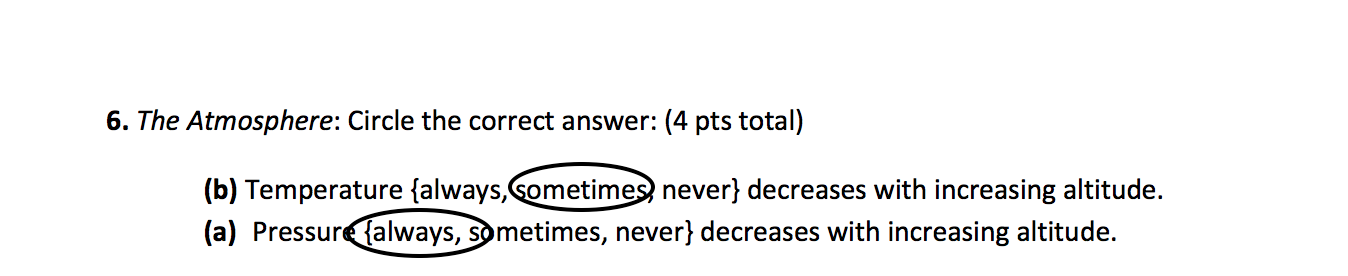
\includegraphics[width=\textwidth]{Q6.png} 
        \end{figure}

\hrulefill


        \textbf{Problem 7:}

        a) Actual lapse rate $=-dT/dz=(290K-220K)/(10km)=-7K/km$

        b) 7 is closer to 6 (wet) than to 9.8 (dry), so it is closer to the wet rate.






        
        % \begin{figure}[h]
        %     \centering
        %       \includegraphics[width=0.5\textwidth]{FIGURE2.png}
        %       \caption{Present value cost plotted with the cost function.}
        %   \end{figure}

    \end{flushleft}

 


\end{document}